%
% differenzen.tex
%
% (c) 2017 Prof Dr Andreas Müller
%
\documentclass[tikz]{standalone}
\usepackage{times}
\usepackage{txfonts}
\usepackage{pgfplots}
\usepackage{csvsimple}
\usetikzlibrary{arrows,intersections}
\begin{document}
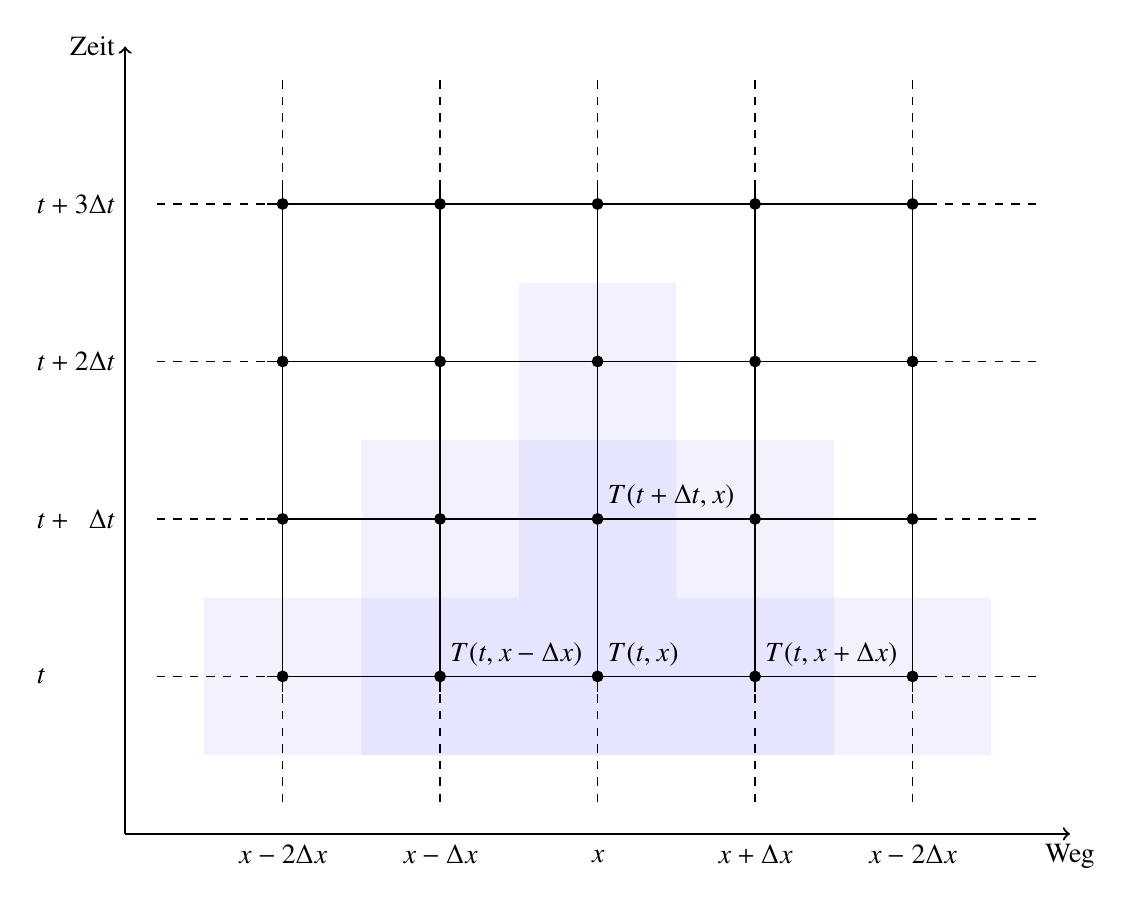
\begin{tikzpicture}[thick,scale=2]

\fill[color=blue!5] (-0.5,-0.5)--(4.5,-0.5)--(4.5,0.5)--(3.5,0.5)--(3.5,1.5)--(2.5,1.5)--(2.5,2.5)--(1.5,2.5)--(1.5,1.5)--(0.5,1.5)--(0.5,0.5)--(-0.5,0.5)--cycle;

\fill[color=blue!10] (0.5,-0.5)--(3.5,-0.5)--(3.5,0.5)--(2.5,0.5)--(2.5,1.5)--(1.5,1.5)--(1.5,0.5)--(0.5,0.5)--cycle;

\foreach \xcoord in {0,...,4} {
	\foreach \ycoord in {0,...,3} {
		\draw[fill=black] ({\xcoord},{\ycoord}) circle[radius=0.03] {};
	}
}
\foreach \xcoord in {0,...,4} {
	\draw[line width=0.5] (\xcoord,-0.1)--(\xcoord,3.1);
	\draw[line width=0.5,dashed] (\xcoord,-0.8)--(\xcoord,-0.1);
	\draw[line width=0.5,dashed] (\xcoord,3.1)--(\xcoord,3.8);
}

\foreach \ycoord in {0,...,3} {
	\draw[line width=0.5] (-0.1,\ycoord)--(4.1,\ycoord);
	\draw[line width=0.5,dashed] (-0.8,\ycoord)--(-0.1,\ycoord);
	\draw[line width=0.5,dashed] (4.1,\ycoord)--(4.8,\ycoord);
}

\node at (1,0) [above right] {$T(t,x-\Delta x)$};
\node at (2,0) [above right] {$T(t,x)$};
\node at (3,0) [above right] {$T(t,x+\Delta x)$};
\node at (2,1) [above right] {$T(t+\Delta t,x)$};

\node at (-1,0) [left] {$t\phantom{\mathstrut+2\Delta t}$};
\node at (-1,1) [left] {$t+\phantom{2}\Delta t$};
\node at (-1,2) [left] {$t+2\Delta t$};
\node at (-1,3) [left] {$t+3\Delta t$};

\node at (0,-1) [below] {$x-2\Delta x\mathstrut$};
\node at (1,-1) [below] {$x-\Delta x\mathstrut$};
\node at (2,-1) [below] {$x\mathstrut$};
\node at (3,-1) [below] {$x+\Delta x\mathstrut$};
\node at (4,-1) [below] {$x-2\Delta x\mathstrut$};

\draw[->] (-1,-1)--(5.0,-1) coordinate[label = {below:$\hbox{Weg}$}];
\draw[->] (-1,-1)--(-1,4.0) coordinate[label = {left:$\hbox{Zeit}$}];

\end{tikzpicture}
\end{document}
